\chapter{Team Member Review and Comment}
\label{chap:team_review}

% Team photograph (template). Uses figures/team_photo.jpg when it exists, otherwise a placeholder box.
\begin{figure}[H]
    \centering
    \IfFileExists{figures/team_photo.jpg}{%
        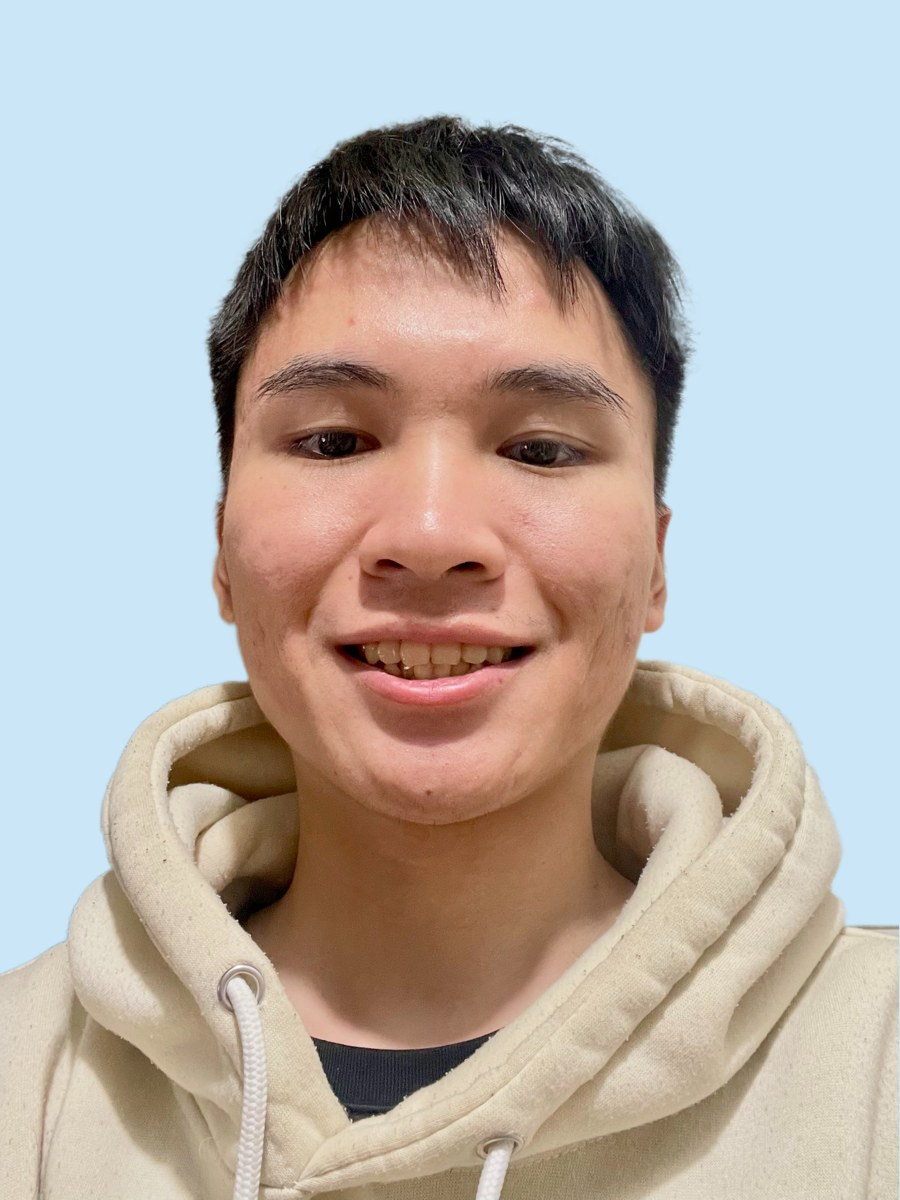
\includegraphics[height=7.5cm]{figures/team_photo.jpg}%
    }{%
        \fcolorbox{SamsungGray}{white}{\parbox[c][6.2cm][c]{0.83\textwidth}{\centering
            {\sffamily\Large\color{SamsungGray}< ATTACH A TEAM PICTURE HERE >}\\[8pt]
            {\sffamily\small\color{SamsungGray}Save the photo as figures/team\_photo.jpg and rebuild the report.}}}%
    }
    \caption{Team member --- \memberOne}
    \label{fig:team_photo}
\end{figure}

\noindent
\begin{table}[H]
    \centering
    \caption{Individual Team Member Reviews and Comments}
    \label{tab:team_member_comments}
    \renewcommand{\arraystretch}{2.0}
    \arrayrulecolor{SamsungGray}
    \begin{tabularx}{\textwidth}{|>{\raggedright\arraybackslash\sffamily}p{3.2cm}|>{\raggedright\arraybackslash}X|}
        \hline
        \rowcolor{SamsungLightBlue}
        \multicolumn{1}{|c|}{\sffamily\bfseries\color{SamsungDarkGray}NAME} & 
        \multicolumn{1}{c|}{\sffamily\bfseries\color{SamsungDarkGray}REVIEW and COMMENT} \\
        \hline
        \textbf{\memberOne} & \textbf{Role:} Project owner (individual project): problem definition, data, model, evaluation, application and report.\newline
\textbf{Tasks:} Defined the task and pre-registered the hypotheses; converted and cleaned UA-DETRAC and built the camera-location split; designed, implemented and trained GapLink-Lite and the baselines C-1\dots C-4; ran the locked Phase-1 test and the live Phase-2 evaluation; tuned the model for YOLOv8n; built the demonstration consoles (first a side-by-side GapLink-VMS, then the GapLink Live upload console) and selected and checked the demonstration clips against ground truth; wrote the automated tests and the report.\newline
\textbf{Self-review:} The main result is solid and verifiable: two of three pre-registered hypotheses and the protocol check pass, and the advantage over the Kalman association survives a live detector. The weak points are the failed calibration hypothesis (H2), the live wrong-link rate above the 5\% target, and the second Phase-1 test run after a data fix, all reported openly.\newline
\textbf{Peer comment:} Not applicable (individual project).\\
        \hline
    \end{tabularx}
\end{table}
